\documentclass{beamer}
\mode<presentation>
\usepackage{amsmath}
\usepackage{amssymb}
%\usepackage{advdate}
\usepackage{graphicx}
\graphicspath{{../Figs/}}
\usepackage{adjustbox}
\usepackage{subcaption}
\usepackage{enumitem}
\usepackage{multicol}
\usepackage{mathtools}
\usepackage{listings}
\usepackage{url}
\def\UrlBreaks{\do\/\do-}
\usetheme{Boadilla}
\usecolortheme{lily}
\setbeamertemplate{footline}
{
  \leavevmode%
  \hbox{%
  \begin{beamercolorbox}[wd=\paperwidth,ht=2.25ex,dp=1ex,right]{author in head/foot}%
    \insertframenumber{} / \inserttotalframenumber\hspace*{2ex} 
  \end{beamercolorbox}}%
  \vskip0pt%
}
\setbeamertemplate{navigation symbols}{}

\providecommand{\nCr}[2]{\,^{#1}C_{#2}} % nCr
\providecommand{\nPr}[2]{\,^{#1}P_{#2}} % nPr
\providecommand{\mbf}{\mathbf}
\providecommand{\pr}[1]{\ensuremath{\Pr\left(#1\right)}}
\providecommand{\qfunc}[1]{\ensuremath{Q\left(#1\right)}}
\providecommand{\sbrak}[1]{\ensuremath{{}\left[#1\right]}}
\providecommand{\lsbrak}[1]{\ensuremath{{}\left[#1\right.}}
\providecommand{\rsbrak}[1]{\ensuremath{{}\left.#1\right]}}
\providecommand{\brak}[1]{\ensuremath{\left(#1\right)}}
\providecommand{\lbrak}[1]{\ensuremath{\left(#1\right.}}
\providecommand{\rbrak}[1]{\ensuremath{\left.#1\right)}}
\providecommand{\cbrak}[1]{\ensuremath{\left\{#1\right\}}}
\providecommand{\lcbrak}[1]{\ensuremath{\left\{#1\right.}}
\providecommand{\rcbrak}[1]{\ensuremath{\left.#1\right\}}}
\theoremstyle{remark}
\newtheorem{rem}{Remark}
\newcommand{\sgn}{\mathop{\mathrm{sgn}}}
\providecommand{\abs}[1]{\left\vert#1\right\vert}
\providecommand{\res}[1]{\Res\displaylimits_{#1}} 
\providecommand{\norm}[1]{\lVert#1\rVert}
\providecommand{\mtx}[1]{\mathbf{#1}}
\providecommand{\mean}[1]{E\left[ #1 \right]}
\providecommand{\fourier}{\overset{\mathcal{F}}{ \rightleftharpoons}}
%\providecommand{\hilbert}{\overset{\mathcal{H}}{ \rightleftharpoons}}
\providecommand{\system}[1]{\overset{\mathcal{#1}}{ \longleftrightarrow}}
%\providecommand{\system}{\overset{\mathcal{H}}{ \longleftrightarrow}}
	%\newcommand{\solution}[2]{\textbf{Solution:}{#1}}
%\newcommand{\solution}{\noindent \textbf{Solution: }}
\providecommand{\dec}[2]{\ensuremath{\overset{#1}{\underset{#2}{\gtrless}}}}
\newcommand{\myvec}[1]{\ensuremath{\begin{pmatrix}#1\end{pmatrix}}}
\let\vec\mathbf

\lstset{
%language=C,
frame=single, 
breaklines=true,
columns=fullflexible
}

\numberwithin{equation}{section}


\begin{document}


\title{4.13.71}
\author{AI25BTECH11002 - Ayush Sunil Labhade}
{\let\newpage\relax\maketitle}


\textbf{Question:}

If the vectors \(a \hat{i} + \hat{j} + \hat{k}\), \(\hat{i} + b \hat{j} + \hat{k}\) and \(\hat{i} + \hat{j} + c \hat{k}\) \((a \neq b \neq c \neq 1)\) are co-planar, then
the value of \(\dfrac{1}{1-a} + \dfrac{1}{1-b} + \dfrac{1}{1-c} = \dotsb\).

\textbf{Solution:}

The vectors are coplanar if they are linearly dependent, i.e., the matrix formed by them has rank less than 3.

Let \(\vec{u} = a \hat{i} + \hat{j} + \hat{k}\), \(\vec{v} = \hat{i} + b \hat{j} + \hat{k}\), \(\vec{w} = \hat{i} + \hat{j} + c \hat{k}\).

Form the matrix
\begin{align}
	\vec{M} = \myvec{a & 1 & 1 \\ 1 & b & 1 \\ 1 & 1 & c}.
\end{align}

For rank $<3$, perform row reduction to find the condition.

After row reducing the matrix:

\begin{align}
\myvec{1 & b & 1 \\ 0 & 1 - ab & 1 - a \\ 0 & 1 - b & c - 1}.
\end{align}

Assuming \(1 - ab \neq 0\) (consistent with \(a \neq b \neq 1\)), to eliminate the second column in $R_3$, compute the multiplier \(k = \frac{1 - b}{1 - ab}\).

Replace $R_3$ with $R_3$ $-$ \(k\) $R_2$:

The second entry becomes \(1 - b - k (1 - ab) = 0\) by construction.
The third entry becomes \(c - 1 - k (1 - a) = 0\) for the row to be zero (ensuring rank 2).

For rank $<3$, the third entry must be zero:
\begin{align}
c - 1 = k (1 - a) = \frac{1 - b}{1 - ab} (1 - a).
\end{align}

Solving for \(c\):
\begin{align}
c &= 1 + \frac{(1 - b)(1 - a)}{1 - ab} = \frac{1 - ab + (1 - a)(1 - b)}{1 - ab} = \frac{2 - a - b}{1 - ab}.
\end{align}

Now, compute \(\frac{1}{1 - a} + \frac{1}{1 - b} + \frac{1}{1 - c}\).

First, find \(1 - c\):
\begin{align}
1 - c = 1 - \frac{2 - a - b}{1 - ab} = \frac{-(1 - a)(1 - b)}{1 - ab}.
\end{align}

Thus,
\begin{align}
\frac{1}{1 - c} = \frac{1 - ab}{-(1 - a)(1 - b)} = -\frac{1 - ab}{(1 - a)(1 - b)}.
\end{align}

The sum is:
\begin{align}
\frac{1}{1 - a} + \frac{1}{1 - b} - \frac{1 - ab}{(1 - a)(1 - b)} &= \frac{(1 - b) + (1 - a) - (1 - ab)}{(1 - a)(1 - b)} \\
&= \frac{(1 - a)(1 - b)}{(1 - a)(1 - b)} = 1.
\end{align}

Thus, the value is 1.


Graph:
\begin{figure}[H]
    \centering
    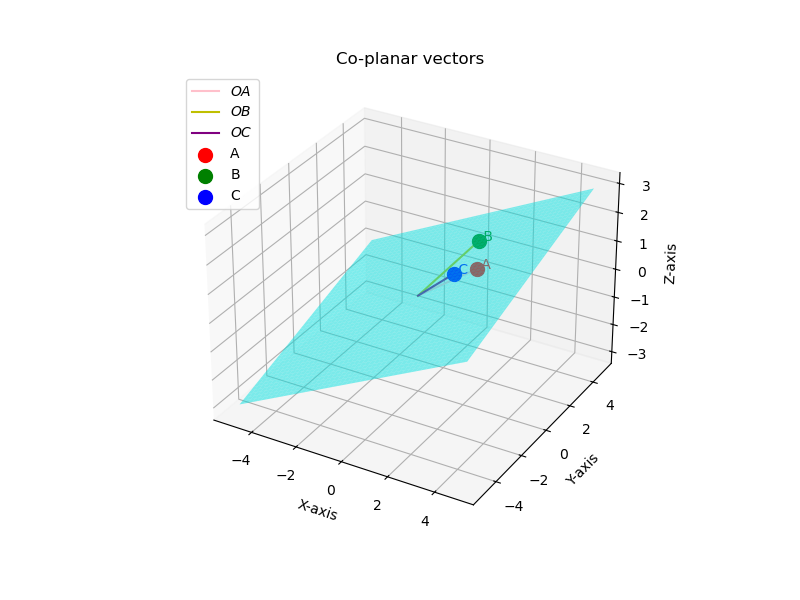
\includegraphics[scale=0.5]{plot}
    \caption{}
    \label{fig:plot}
\end{figure}
\end{document}
